\documentclass{beamer}
\usetheme{Frankfurt}
\usepackage[utf8]{inputenc}
\usepackage{charter}
\usepackage{tikz}
\usepackage{graphicx}
\usepackage{amsmath}
\usepackage{amssymb}
\usepackage{listings}
\usepackage{animate}
\beamertemplatenavigationsymbolsempty

%% Title slide formatting %%

\pgfdeclareimage[width=\paperwidth]{titlebackground}{Images/title-slide-background.png}
\setbeamerfont{subtitle}{size=\tiny}
\setbeamertemplate{endpage}{
	\begin{picture}(0,0)
		\scalebox{1.01}{
		\put(-28.5,-163){%
			\pgfuseimage{titlebackground}
		}
		}
		\put(0,-115){%
			\begin{minipage}[b][4.5cm][t]{0.5\textwidth}
				\color{white}
				\usebeamerfont{title}
				{\textbf{Thank Your} \\ \textbf{For You Attention !}}
			\end{minipage}
		}
	\end{picture}
}
\setbeamertemplate{title page}{
	\begin{picture}(0,0)
		\scalebox{1.01}{
			\put(-28.5,-163){%
				\pgfuseimage{titlebackground}
			}
		}
		\put(0,-75){%
			\begin{minipage}[b][4.5cm][t]{0.5\textwidth}
				\color{white}
				\usebeamerfont{title}
				{\inserttitle\\[0.9cm]}
				\usebeamerfont{subtitle}
				{\insertauthor\par}
				{\insertinstitute\\[0.3cm]}
				{\insertdate}
			\end{minipage}
		}
	\end{picture}
}


%% General slide formatting %%

\definecolor{oxfordblue}{RGB}{4,30,66}

\pgfdeclareimage[width=0.9cm]{oxfordlogo}{Images/oxford-logo.png}
\pgfdeclareimage[width=1cm]{mathslogo}{Images/mathematics-logo.png}
\pgfdeclareimage[width=0.9cm]{pizzalogo}{Images/pizza-logo.png}

\setbeamertemplate{headline}
{%
	\begin{picture}(0,0)
		\put(314,-50){%
			\pgfuseimage{oxfordlogo}
		}
		\put(20,-55){%
			\rule{320pt}{0.4pt}
		}
	\end{picture}
}

\setbeamertemplate{frametitle}
{%
	\begin{picture}(0,0)
		\put(-8,-20){%
			\normalsize\textbf{\color{oxfordblue}\insertframetitle}
		}
		\put(-7,-25){%
			\small\color{oxfordblue}\insertframesubtitle
		}
	\end{picture}
}

\setbeamertemplate{footline}
{%
	\begin{picture}(0,0)
		\put(20,30){%
			\rule{320pt}{0.4pt}
		}
		\put(20,14){%
			\pgfuseimage{mathslogo}
		}
		\put(100,14){%
			\color{oxfordblue}\insertshortdate
		}
		\put(160,14){%
			\color{oxfordblue}\insertshorttitle
		}
		\put(337,14){%
			\color{oxfordblue}\insertframenumber
		}
	\end{picture}%
}
\setbeamercolor{block title}{bg=oxfordblue!30,fg=black}

\definecolor{codegreen}{rgb}{0,0.6,0}
\definecolor{codegray}{rgb}{0.5,0.5,0.5}
\definecolor{codepurple}{rgb}{0.58,0,0.82}
\definecolor{backcolour}{rgb}{0.95,0.95,0.92}

\lstdefinestyle{mystyle}{
	%backgroundcolor=\color{backcolour},   
	commentstyle=\color{codegray},
	keywordstyle=\color{oxfordblue},
	numberstyle=\tiny\color{codegray},
	stringstyle=\color{codegreen},
	basicstyle=\ttfamily\footnotesize,
	breakatwhitespace=false,         
	breaklines=true,                 
	captionpos=b,                    
	keepspaces=true,                 
	numbers=left,                    
	numbersep=5pt,                  
	showspaces=false,                
	showstringspaces=false,
	showtabs=false,                  
	tabsize=2
}

\lstset{style=mystyle}

%% Information (author, title, etc.) %%

\title[Firedrake-NETGEN]{Firedrake-NETGEN Integration: New Features} % short title for footer
\author%
{%
	\sc{P. E. Farrell} *, \sc{S. Zampini}$\;\dagger$, \underline{\sc{U. Zerbinati}} *\\
}
\institute%
{%
	* \textit{Mathematical Institute}\\
	\;\textit{University of Oxford}\\
	\\
	$\;\dagger\;$\textit{Extreme Computing Research Center}\\
	\;\textit{King Abdullah University of Science and Technology}
}

\date[Firedrake 2023]{Firedrake User Meeting, Great Missenden, 13th of September 2023} % short date for footer



%% Content of slides %%

\begin{document}
	\begin{frame}[plain]
		\titlepage
	\end{frame}
	%
	\begin{frame}
		\frametitle{Solving a Partial Differential Equation}
		When solving a partial differential equation the following macro steps can be identified:
		$\newline$
		\begin{itemize}
			\item[\color{oxfordblue}$\blacktriangleright$] Geometrical modelling,
			\item[\color{oxfordblue}$\blacktriangleright$] Meshing,
			\item[\color{purple}$\blacktriangleright$] Discretising a PDE,
			\item[\color{purple}$\blacktriangleright$] Solving the linear or nonlinear system.
		\end{itemize}
		$\newline$
		We aim to allow the Firedrake user to do all the steps above described in a single script.
	\end{frame}
	\begin{frame}
		\frametitle{Why NetGen?}
		\framesubtitle{}
		NetGen is an advancing front 2D/3D-mesh generator, with many interesting features. Among the most important:
		$\newline$
		\begin{itemize}
			\item[\color{oxfordblue}$\blacktriangleright$] Python wrapping (through pybind11),
			\item[\color{oxfordblue}$\blacktriangleright$] Multiple ways of describing the geometry to be meshed, i.e. its builtin \textbf{Constructive Solid Geometry} (\textbf{CSG}) and the \textbf{Open Cascade Technology} (\textbf{OCCT}) geometry kernel,
			\item[\color{oxfordblue}$\blacktriangleright$] Supports \textbf{adaptive mesh refinement} (also anisotropic mesh refinement).
			\item[\color{oxfordblue}$\blacktriangleright$] Supports \textbf{high-order} meshes for curved geometries.
		\end{itemize}
	\end{frame}
	\begin{frame}
		\frametitle{Getting Started -- Installing NetGen}
		$\newline$
			\begin{block}{Install NetGen using Firedrake scripts}
				\begin{center}
				\lstinline! python3 firedrake-install --netgen !
				\\
				\lstinline! python3 firedrake-update --netgen !
				\end{center}
			\end{block}
			\begin{alertblock}{PETSc}
				If you are using an external PETSc installation, it should be updated to include commit \texttt{654059db}.
			\end{alertblock}
			\begin{alertblock}{NetGen}
				If you are interested in \textbf{anisotropic mesh refinement}, please install, \texttt{https://github.com/UZerbinati/netgen.git}
			\end{alertblock}
	\end{frame}
	\begin{frame}
		\frametitle{Firedrake-NETGEN Integration: Old Features}
		\framesubtitle{}
		$\newline$
		Some of the old features of the Firedrake-NETGEN integration are:
		\begin{itemize}
			\item[\color{oxfordblue}$\blacktriangleright$] Describing the geometry to be meshed using \textbf{Open Cascade Technology} geometry kernel.
			\item[\color{oxfordblue}$\blacktriangleright$] Using \textbf{NETGEN} as a mesh generator in Firedrake, for \textbf{linear} meshes.
			\item[\color{oxfordblue}$\blacktriangleright$] Marking subregions of the geometry for \textbf{finer meshing}.
			\item[\color{oxfordblue}$\blacktriangleright$] \textbf{Adaptive mesh refinement}, this feature can be accessed using the \texttt{refine\_marked\_elements} method.
		\end{itemize}
	\end{frame}
	\begin{frame}
		\frametitle{ngsPETSc -- A new component of NGSolve}
		\framesubtitle{}
		\textbf{ngsPETSc} is a new component of the NGSolve library, which allows to use PETSc as a linear algebra backend for NGSolve.
		In particular thanks to the \textbf{NETGEN-DMPlex} interface it is possible NETGEN mesh in Firedrake.
		$\newline$
		\begin{itemize}
			\item[\color{oxfordblue}$\blacktriangleright$] Less code to maintain on the Firedrake side and additional features for the \textbf{NETGEN-DMPlex} interface. 
			\item[\color{oxfordblue}$\blacktriangleright$] No need to install the full NGSolve library, for most of the features here presented only NETGEN will suffice.
		\end{itemize}
	\end{frame}
	\begin{frame}
		\frametitle{Firedrake-NETGEN Integration: New Features}
		\framesubtitle{}
		Some of the old features of the Firedrake-NETGEN integration are:
		$\newline$
		\begin{itemize}
			\item[\color{oxfordblue}$\blacktriangleright$] Using \textbf{NETGEN} as a mesh generator in Firedrake, for \textbf{high-order} meshes.
			\item[\color{oxfordblue}$\blacktriangleright$] Support for \textbf{anisotropic} mesh refinement, using NetGen \texttt{ZRefinement} and \texttt{HPRefinement} methods.
			\item[\color{oxfordblue}$\blacktriangleright$] Using \textbf{PETSc Transformation} for \textbf{Alfeld} and \textbf{Powell-Sabin} splits and \textbf{quadrilateral} meshes.
		\end{itemize}
	\end{frame}
	\begin{frame}
		\frametitle{Open Cascade -- High Order Meshes}
		\begin{minipage}{0.7\textwidth}
			$\newline$
			\lstinputlisting[language=Python,firstline=6]{Codes/test_work_plane.py}
		\end{minipage}
		\begin{minipage}{0.25\textwidth}
			\vspace{-0.3cm}
			\begin{figure}
				\centering
				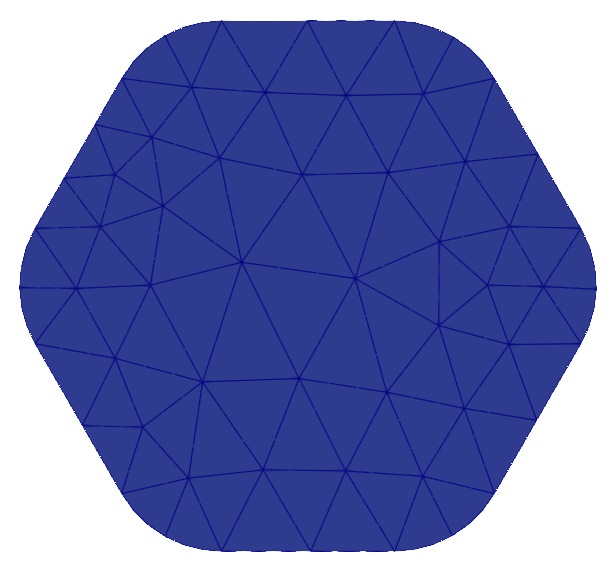
\includegraphics[scale=0.15]{Figures/wp.png}
			\end{figure}
		\end{minipage}
	\end{frame}
	\begin{frame}
		\frametitle{Open Cascade 3D -- High Order Meshes}
		\begin{minipage}{0.7\textwidth}
			$\newline$
			\lstinputlisting[language=Python,firstline=6]{Codes/test_sphere.py}
		\end{minipage}
		\begin{minipage}{0.25\textwidth}
			\vspace{-0.3cm}
			\begin{figure}
				\centering
				\includegraphics<1>[scale=0.15]{Figures/sphere.png}
				\includegraphics<2>[scale=0.15]{Figures/spherePoisson.png}
			\end{figure}
		\end{minipage}
	\end{frame}
	\begin{frame}
		\frametitle{Constructive Solid Geometry -- High Order Meshes}
		\begin{minipage}{0.7\textwidth}
			$\newline$
			\lstinputlisting[language=Python,firstline=6,lastline=15]{Codes/test_plate.py}
		\end{minipage}
		\begin{minipage}{0.25\textwidth}
			\vspace{-0.3cm}
			\begin{figure}
				\centering
				\includegraphics<1>[scale=0.15]{Figures/plate.png}
			\end{figure}
		\end{minipage}
	\end{frame}
	\begin{frame}
		\frametitle{Anisotropic Mesh Refinement -- Singular Vertex}
		\begin{minipage}{0.7\textwidth}
			$\newline$
			\lstinputlisting[language=Python,firstline=7,lastline=18]{Codes/test_hprefine_vertex.py}
		\end{minipage}
		\begin{minipage}{0.25\textwidth}
			\vspace{-0.3cm}
			\begin{figure}
				\centering
				\includegraphics<1>[scale=0.1]{Figures/cylinderVertex.png}
				$\newline$
				$\newline$
				\includegraphics<1>[scale=0.1]{Figures/cylinderVertexZoom.png}
			\end{figure}
		\end{minipage}
	\end{frame}
	\begin{frame}
		\frametitle{Anisotropic Mesh Refinement -- Singular Edge}
		\begin{minipage}{0.7\textwidth}
			$\newline$
			\lstinputlisting[language=Python,firstline=6,lastline=17]{Codes/test_hprefine_edge.py}
		\end{minipage}
		\begin{minipage}{0.25\textwidth}
			\vspace{-0.3cm}
			\begin{figure}
				\centering
				\includegraphics<1>[scale=0.15]{Figures/cylinderEdge.png}
			\end{figure}
		\end{minipage}
	\end{frame}
	\begin{frame}
		\frametitle{Anisotropic Mesh Refinement -- Z Refinement}
		\begin{minipage}{0.7\textwidth}
			$\newline$
			\lstinputlisting[language=Python,firstline=7,lastline=18]{Codes/test_zrefine.py}
		\end{minipage}
		\begin{minipage}{0.25\textwidth}
			\vspace{-0.3cm}
			\begin{figure}
				\centering
				\includegraphics<1>[scale=0.2]{Figures/ZRefine.png}
			\end{figure}
		\end{minipage}
	\end{frame}
	\begin{frame}
		\frametitle{PETSc Transformation -- Alfeld Split}
		\begin{minipage}{0.7\textwidth}
			$\newline$
			\lstinputlisting[language=Python,firstline=7,lastline=16]{Codes/test_alfeld.py}
		\end{minipage}
		\begin{minipage}{0.25\textwidth}
			\vspace{-0.3cm}
			\begin{figure}
				\centering
				\includegraphics<1>[scale=0.13]{Figures/alfeld.png}
			\end{figure}
		\end{minipage}
	\end{frame}
	\begin{frame}
		\frametitle{Curved Alfeld Split}
		\begin{minipage}{0.7\textwidth}
			$\newline$
			\lstinputlisting[language=Python,firstline=8,lastline=18]{Codes/test_curved_alfeld.py}
		\end{minipage}
		\begin{minipage}{0.25\textwidth}
			\vspace{-0.3cm}
			\begin{figure}
				\centering
				\includegraphics<1>[scale=0.08]{Figures/curvedAlfeld.png}
			\end{figure}
		\end{minipage}
	\end{frame}
	\begin{frame}
		\frametitle{PETSc Transformation -- Quadrilateral Split}
		\begin{minipage}{0.7\textwidth}
			$\newline$
			\lstinputlisting[language=Python,firstline=6,lastline=15]{Codes/test_quad.py}
		\end{minipage}
		\begin{minipage}{0.25\textwidth}
			\vspace{-0.3cm}
			\begin{figure}
				\centering
				\includegraphics<1>[scale=0.15]{Figures/plateQuad.png}
			\end{figure}
		\end{minipage}
	\end{frame}
	\begin{frame}
		\frametitle{Conclusion}
		$\newline$
		\begin{itemize}
			\item[\color{oxfordblue}$\blacktriangleright$] Improve support for \textbf{quadrilateral elements}, and consider \textbf{hexahedral elements}. 
			\item[\color{oxfordblue}$\blacktriangleright$] Mesh \textbf{hierarchy awareness}, using Firedrake \texttt{HierarchyBase} class.
			\item[\color{oxfordblue}$\blacktriangleright$] Support \textbf{``snap back''}, to OCCT geometry, thanks to PETSc OCC awareness.
			\item[\color{oxfordblue}$\blacktriangleright$] Support for MFEM \textbf{GLVIS} mesh and solution live display, thanks to PETSc-GLVIS interface.
		\end{itemize}
	\end{frame}
\end{document}
